% MUST use a4paper option
% MAY use twoside, smaller font, and other class
\documentclass[swedish, a4paper,12pt]{article}
%\documentclass[swedish,12pt]{<class>}
% Use UTF-8 encoding in input files
\usepackage[utf8x]{inputenc}
% TODO: If you are writing in English, un-comment the following line:
\usepackage[swedish, english]{babel}
% Use the template for thesis reports
\usepackage{UppsalaExjobb}
\usepackage{float}

% Useful font packages for maths and symbols
\usepackage{amssymb,amsmath,amsthm,amsfonts}

% for nice code listings
\usepackage{listings}
%\usepackage[hyphens]{url}
%\usepackage{hyperref}


\usepackage{url}
% Designval: per default används styckesindrag, men ibland blir det snyggare/mer lättläst med tomrad mellan stycken. Det åstadkoms av de följande raderna.
% Tycker ni om styckesindrag mera, kommentera bort nästa två rader.
\parskip=0.8em
\parindent=0mm

\begin{document}

% Set title, and subtitle if you have one
\title{Positioneringssystem för aktivitetsbaserade arbetsplatser} % och uppsatsmetodik
% Use this if you have a subtitle
%\subtitle{Really Exciting Stuff}
% Set author names, separated by "\\ " (don't forget the space)
% List authors alphabetically by last name (unless someone did significantly more/less)
\author{Albin Hjelm \\ Sebastian Gustafsson \\ Alexander Backlund}
% Set the date and year - use the right language!
\date{\begin{otherlanguage}{swedish}  %\foreignlanguage doesn't seem to affect \today?
\today
\end{otherlanguage}}

% Only need to set the year if it differs from the current year
%\year=2018

% Ange handledare, ämnesgranskare, examinator om dessa finns
% Extern handledare: t.ex på företag ni arbetat med?
%\exthandledare{NN}
% Intern handledare
\handledare{Lisa Lagom och Björn Victor}
% Ämnesgranskare används inte på Självständigt arbete i IT
%\reviewer{NN}
% På Självständigt arbete i IT är detta BV
\examinator{Björn Victor}

% Programnamn på svenska och engelska
\progname{Civilingenj{\"o}rsprogrammet i informationsteknologi}{Computer and Information Engineering Programme}

% Utgivare
\enhetsnamn{Institutionen för \\ informationsteknologi}
\besoksadress{ITC, Polacksbacken\\ Lägerhyddsvägen 2}
\postadress{Box 337 \\ 751 05 Uppsala}
\hemsida{http:/www.it.uu.se}

% Set the name of the series, and the number in the series
\seriesname{Självständigt arbete i informationsteknologi}
% \seriesname{Uppsatsmetodik}

% OBS: Gäller bara exjobb i årskurs 5
% Get a series number, e.g. from Studentservice Ångström
%\seriesnumber{UPTEC IT16~0xx}
% Use the appropriate ISSN for the series
%\issn{ISSN 1401-5749}
% Usually this is where it is printed
%\printer{Ångströmlaboratoriet, Uppsala universitet}

% This creates the title page
\maketitle

% Change to frontmatter style (e.g. roman page numbers)
\frontmatter

\begin{abstract}
% Abstract in English, about 10-20 lines. Do not use references; do not use formulas if they can be avoided.
% \begin{enumerate}
% \item What is the problem/issue/subject?
% \item How was the problem solved/attacked?
% \item What are the results, how well was the problem solved?
% \item How good are the results, how useful are they?
% \end{enumerate}
% The abstract should be understandable without reading the whole report (and the rest of the report should be understandable without reading the abstract). You can reuse text/phrases from the Introduction.
Many companies and organisations nowadays chose to transfer from an office structure consisting of employee dedicated offices into having a more open and office free structure. With that transition some difficulties occur in locating coworkers when you want to discuss something since they now have the opportunity to choose workplace more freely. %work related concerns with%.
 Beacause of this, employees looses productivity and spends unnecessary time and energy on locating coworkers. This project's' intent is to make this transition easy, non time consuming and available only using existing information and technology. This is to be provided via a location platform at which users can locate their co-workers.
\end{abstract}
\begin{sammanfattning}
% Sammanfattning på svenska. Se till att det står samma saker i det svenska och det engelska abstractet.
% \begin{enumerate}
% \item Vad är problemet, ämnet?
% \item Hur angreps/löstes problemet?
% \item Vad är resultaten, hur väl löstes problemet?
% \item Hur bra blev resultaten, hur användbara är de?
% \end{enumerate}
%
% Ca 10-20 rader. Använd inte referenser; ej heller formler om det går att undvika.
%
% Abstract ska vara förståeligt utan att läsa resten av rapporten, och resten av rapporten ska kunna läsas utan att läsa abstract. Man kan återanvända text från introduktionen.
Många företag och organisationer nuförtiden väljer att övergå från en kontorsstruktur bestående av dedikerade kontorsplatser för var och en av medarbetarna till en öppnare och mer kontorsfri struktur. Med den övergången tillkommer vissa problem med att hitta de medarbetare som du vill träffa och diskutera med eftersom de nu har möjlighet att välja arbetsplats friare. På grund av detta tappar de anställda i produktivitet eftersom de behöver spendera onödig tid på att lokalisera sina kollegor. En kontorsstruktur där medarbetarna väljer arbetsplats utifrån arbetsuppgift kallas för en aktivitetsbaserad arbetsplats. Det här projektets intention är att göra övergången till en aktivitetsbaserad arbetsplats enkel, icke tidskrävande och möjlig genom att endast använda befintlig teknik och information på arbetsplatsen. Medarbetarnas position kommer presenteras via en lokaliseringsplattform där varje användare enkelt kan lokalisera sina medarbetare.

 %%förlytta deras verksamhet från kontorsbaserad till en mer kontorsfri miljö. Med den övergången tillkommer vissa problem med att hitta medarbetare för att kunna diskutera arbetsrelaterade saker. På grund av det här tappar de anställda i produktivitet, eftersom de behöver spendera för mycket tid på att lokalisera sina kollegor. Detta projektets intention är att göra övergången enkel, icke tidskrävande och möjlig genom att endast använda befinntlig information och teknik. Vilket ges via en lokaliserings plattform som användare kan lokalisera sina medarbetare.
\end{sammanfattning}

% Innehållsförteckningen här.
\tableofcontents

% Här kan man också ha \listoffigures, \listoftables

\cleardoublepage


% Change to main matter style (arabic page numbers, reset page numbers)
\mainmatter

% Here comes the text of the report.

\iffalse
\section*{Hur ni använder detta malldokument}
Titta i källdokumentet för diverse inställningar för författare, titel, etc.

\emph{OBSERVERA} att de ``fasta fält'' som blir på svenska (trots att ni ställt in engelska med \texttt{babel}), som Examinator, Handledare, datum på framsidan osv, \emph{ska} vara på svenska oavsett språk i rapporten. Abstract ska alltid vara på engelska, medan Sammanfattning alltid ska vara på svenska.

I flera appendix finns mer info som inte gäller rapportstrukturen.

I era inlämningar, ta bort (eller kommentera bort) malltexten (beskrivningen av vad som ska stå), men behåll gärna tomma huvudrubriker. Ta också bort mall-appendix.

\subsection*{Generellt}
Varje numrerat avsnitt ska finnas med i er slutrapport, om inget annat anges.
Välj rubrik på svenska eller engelska beroende på ert valda rapportspråk.

Glöm inte att läsa kurslitteraturen~\cite{dawson:projects-in-computing,dawson:projects-in-computing-old}.
\fi

% \subsection*{Uppdateringar av detta dokument}
% \begin{description}
% \item[2016-05-16]\mbox{}\\

% \end{description}


\section*{Att göra}
Tredje utkast: systemstruktur, metoder.

\newpage %%%%%%%%%%%%%%%% OBS! Ta bort allt mellan \mainmatter och här (inkl \newpage) i slutversionen (men inte \mainmatter)

\section{Introduktion}
\iffalse Beskriv åtminstone samma saker som i abstract, men mer utförligt. Spara tekniska detaljer till senare.

Tänk på att börja introduktionen med en mening eller ännu hellre ett helt stycke som ``fångar'' läsaren och motiverar läsaren att fortsätta läsa.  \emph{Vi har valt att göra ett projekt om X} är relevant för er, men kommer inte att vilja få någon att läsa vidare.  Försök åtminstone få med någon slags bakgrund/kontext och (helst) motivation att fortsätta läsa.  Typ \emph{X är ett programspråk som tagit världen med storm.  Vi vill utforska om man kan kombinera X med Y för att göra\ldots}

Se till att ni \emph{kommer till kritan snabbt} – man vill inte läsa igenom två stycken text innan man får veta vad ni tänker göra i ert projekt.  Börja t.ex. \emph{inte} med att presentera alla idéer ni inte valt – läsaren vill veta vad ni ska göra, inte vad ni inte ska göra.

Översiktlig beskrivning av systemet och dess features ska vara under systemdesign / systemstruktur, inte i introduktionen.

Introduktionen bör vara begriplig för t.ex.~en student i årskursen under, och gärna för en ännu bredare läsarkrets.
\fi

Fler och fler företag och organisationer väljer idag att övergå från kontorsbaserade till aktvitetsbaserade arbetsplatser. Iden med en aktivitetsbaserad arbetsplats är att arbetsytorna öppnas upp och delas in i områden snarare än mindre kontor. Ett problem med denna typ av miljö är att det är svårt att veta vart sina medarbetare befinner sig. Lösningen till problemet är vårat system. Systemet fungerar så att när en medarbetare startar sin dator kommer den att skanna av nätverksinformationen i närheten och bestämma medarbetarens position. Denna position kommer att visas på en hemsida så att andra medarbetare snabbt kan se vart sina kollegor befinner sig. Som användare kommer man även kunna välja att inte visa sin position.

\iffalse
Tidigare var det absolut vanligaste sättet att organisera en arbetsplats att arbetsplatsen uppdelades i kontor och varje medarbetare hade en specifik kontorsplats.
De medarbetare som tidigare var tilldelade ett specifikt kontor
väljer nu istället en tillfällig arbetsyta baserat på vilken som just då
är mest lämplig för att utföra deras arbetsuppgifter.
\bigskip
\newline
Detta skapar i sin tur vissa problem i och med att det blir svårare att veta vart på arbetsplatsen en medarbetare befinner sig då denne inte har någon fast arbetsplats.
Det är detta problem som det här projektet syftar till att lösa.
\fi

\section{Bakgrund}
\subsection{Aktivitetsbaserad verksamhet (ABV)}
Madeleine Stjärne, \iffalse författaren till skriften "Aktivitetsbaserade
arbetsplatser i offentliga sektor"\fi  beskriver aktivitetsbaserade arbetsplatser på så sätt att de erbjuder medarbetare en varierad arbetsmiljö.\cite{ABV} Hon hävdar att syftet med ABV är att medarbetarna inte ska behöva vara bundna till ett specifikt skrivbord utan istället kunna välja den mest ändamålsenliga arbetsplatsen utifrån den aktuella arbetsuppgiften. % variationen för den individa arbetaren.

Då en organisation väljer att övergå till en aktivitetsbaserad arbetsplats
delas arbetsplatsen in i olika miljöer som stödjer de olika arbetsuppgifterna som ska utföras, såväl individuella arbeten som grupparbeten. En sådan uppdelning görs baserat på resultatet av en verksamhetsanalys. I en verksamhetsanalys hur arbetsplates har använts tidigare. De viktigaste parametrarna att undersöka vid en verksamhetsanalys är vilka arbetsuppgifter som utförs, vart de utförs och hur ofta de utförs.\cite{ABV}
Det är vanligt att arbetsplatsen delas upp i olika zoner. Exempel på zoner är tysta zoner och en möteszoner. Medarbetarna söker sig då till den zon de tycker passar bäst för dagens arbete.

Enligt Lisbeth Slunga Järvholm, forskare vid Umeå universitet passar inte ett aktivitetsbaserat kontor alla. Inte alla sortes arbetsuppgifter fungerar optimalt då man lätt kan bli störd. Vissa arbetsuppgifter kräver en högre koncentrationsnivå, vilket kan vara svårt i ett öppet landskap.\cite{passarInteAlla}
%TODO Fördelar med ett aktivitetsbaserat kontor

\subsection{Uppsala Kommun}
Uppsala Kommun agerar i det här projektet extern intressent. De är i ett skede där de övergår till aktivitetsbaserade arbetsplatser på många av deras kontor runt om i Uppsala. Det innebär att %TODO kolla upp antal
ett par tusen personer kommer att kunna välja friare vart de vill utföra sina arbetsuppgifter. Uppsala Kommun har uttryckt ett behov av att deras medarbetare snabbt ska kunna se vart deras kollegor befinner sig. Det är vår förhoppning att de ska kunna utnyttja vårt system för att kunna uppfylla deras behov.

\subsection{Skype for Business}
Skype for Business är ett kommunikationsmedel som används av många företag och organisationer. Skype for Business(SFB) erbjuder funktionalitet såsom realtidssamtal, videomöten och chattfunktioner. SFB kommer med en möjlighet att konfigurera en egen platsdatabas på SFB´s server.\cite{Microsoft-Office} Det är en funktion som har undersökts om den är lämpligt att använda i detta projekt. När SFB´s platsdatabas är populerad med nätverksinformation för varje område på organisationens arbetsplatser kan en medarbetares position bestämmas med hjälp av vilket nätverk medarbetaren är ansluten till. Denna information visas under användarens namn i Skypes användargränssnitt och är då synlig för andra Skypeanvändare i samma SFB-organisation. Detta gör att användare i SFB enkelt kan lokalisera varandra.

Skype erbjuder två olika versioner av tjänsten Skype for Business. Den ena varianten, Skype for Business \textit{Online} är en molnbaserad tjänst som inte kräver några fysiska servrar hos användaren.\cite{SFBonline}
Den andra varianten, Skype for Business \textit{Server} kräver fysiska servrar hos användaren.\cite{SFBserver}. Funktinaliteten för de två olika versionerna skiljer sig delvis åt och intressenten i det här projektet (Uppsala Komun) hade som önskemål att vi skulle undersöka om funktionen med en platsdatabas i SFB var möjligt i deras fall. Uppsala Komun använder Skype for Business Online.

\subsection{Inomhuspositionering}
Inomhuspositionering är jämfört med utomhuspositionering ett problem med fler komplikationer. GPS-tekniken(Global Position System) som ger en mycket liten felmarginal vid utomhuspositionering är sällan användbar för inomhuspositionering. Anledningen är att GPS-tekniken kräver en oblockerad signal till de satelliter som GPS använder sig av för positionsbestämning. \cite{GPS_US_ACCURACY}

I fallet med inomhuspositionering i kombination med en aktivitetsbaserad arbetsplats ser kraven på precision något annorlunda ut jämfört med precisionskraven för utomhuspositionering. Även om GPS-tekniken kan användas för att bestämma en enhets höjd över marken är den inte tillräckligt tillförlitlig då man vill avgöra på vilket våningsplan i en byggnad en enhet befinner sig.

En av skillnaderna är att det vid positionsbestämning inomhus tillkommer en faktor som komplicerar positionsbestämningen. Problemet är att man vid inomhuspositionering måste ta hänsyn till ett visst antal våningsplan i en byggnad. Även om GPS-tekniken skulle kunna leverera lika god precision inomhus som utomhus (i förhållande till ett globalt koordinatsystem) skulle detta vara otillräckligt i och med att informationen inte anger huruvida den fastställda enhetens position befinner sig på våning 1 eller 15.

%\subsection{Dataskyddsförordningen}
%https://www.datainspektionen.se/dataskyddsreformen/dataskyddsforordningen/introduktion-till-dataskyddsforordningen/ TODO: skriv om detta!
\subsection{Icketekniska aspekter vid inomhuspositionering på \\arbetplatser}

\subsubsection{Säkerhetsmässiga aspekter}
Då många företag och organisationer har säkerhetsmässiga överväganden att ta hänsyn till är det viktigt att vårt system inte bidrar till att säkerheten för medarbetarna i en organisation försämras vid användning av vårt system.
Då vårt system har som uppgift att göra det lättare att lokalisera personal på arbetsplatser kan säkerhetsrisker uppstå. Om det är möjligt för utomstående personer att ta del av information om vart personal befinner sig kan det leda till säkerhetsproblem. I Uppsala Komuns fall finns ett konkret exempel på den typen av säkerhetsproblem. Det arbetar många politiker inom Uppsala Komun och politiker är en yrkesgrupp som ofta får motta våld eller hot om våld. Ifall vårt system bidrar till att det går att tillskansa sig deras exakta position utsätter vi eventuellt dem för risker som inte skulle uppstå utan vårt system.

Detta innebär att det i vårt system är viktigt att det är möjligt att välja att inte visa sin position för andra. Det är också viktigt att personer utanför organisationen inte kan ta del av information om vart personal befinner sig.

\newpage
\subsubsection{Etiska aspekter}
Ur ett etiskt perspektiv finns också vissa frågeställningar som blir viktiga att ha i åtanke under systemets utveckling. Ska systemet till exempel göra det möjligt att öka kontrollen över medarbetarna genom att deras position alltid är känd? Är det lämpligt att föra statistik över vart medarbetare befinner sig vid olika tidpunkter?
Målet med vårt system är inte att det ska användas som ett maktmedel utan för att underlätta för medarbetarna.

\subsubsection{General Data Protection Regulation, GDPR}
GDPR är en ny Europeisk Lagstiftning som gäller alla medlemsländer i EU och träder i kraft den 25 maj 2018.
Lagstiftningen regulerar hantering av personuppgifter och har som syfte att stärka individens rättigheter då företag och organisationer hanterar personuppgifter.\cite{GDPRibm}\cite{GDPRdatainspektionen}
Individer har nu rätt att ta ett ärende som gäller personuppgiftshantering till en rättsprocess mot företag som de anser ha brutit mot de krav som GDPR innebär.
Mynidigheten Datainspektionen i Sverige har nu möjlighet att utdela böter till organisationer och företag som de anser bryter mot de nya lagarna. Det högsta bötesbeloppet som kan utdömmas är 4\% eller 20 miljoner Euro.\cite{GDPRibm}

GDPR eller Dataskyddsförordningen på svenska har vissa regler som i Sverige sedan tidigare reglerats i personuppgiftslagen (PUL). De likheter som finns är bland annat kravet på sammtycke och rätten för en individ att få ta del av hur personuppgifter behandlas. PUL utgår den 25 maj 2018 i sin helhet och ersätts av GDPR.\cite{GDPRdatainspektionen}

Några av de viktigaste nyheterna som detta innebär för den enskilda individen är enligt Datainspektionen\cite{GDPRdatainspektionen}:
\begin{itemize}
  \item Dataportabilitet
  \item Konsekvensbedömmning innan hantering
  \item Anmälningsskyldighet för organisatinoen
  \item Dataskyddsombud hos organisationen
  \item Sanktionsavgifter vid överträdelse
  \item Missbruksregeln upphör.
\end{itemize}
\newpage
Nedan föjler Datainspektionens\cite{GDPRdatainspektionen} förtydligande gällande ovan nämnda bergepp.

\textbf{Dataprortabilitet} innebär att individer ska ha rätten att få ut de personuppgifter de lämnat för att kunna flytta de till en annan tjänst.

\textbf{Konsekvensbedömmning} innebär att innan någon planerar att hantera personuppgifter ska det undersökas vilka risker hanteringen skulle kunna innebära för individen och hur dessa risker ska kunna förebyggas.

\textbf{Anmälningsskyldighet} innebär att vid dataintrång eller dataförlust måste de drabbade informeras och an anmälning måste göras till Datainspektionen inom 72 timmar.

\textbf{Dataskyddsombud.} Innebörden av kravet på ett dataskyddsombud är att varje företag eler organisation som hanterar känsliga personuppgifter måste ha ett dataskyddsombud som hanterar frågor gällande dataskydd.

\textbf{Sanktionsavgift} innebär att Datainspektionen vid överträdelse av dessa regler har rätt att utdela böter i förhållande till hur allvarlig lverträdelsen anses vara.

\textbf{Missbruksregeln} är en regel som funnits i PUL och har inneburit att vissa personuppgifter får behandlas så länge de inte anses kunna vara kränkande för någon. Denna regel försvinner i och med att GDPR börjar gälla.

Enligt en av IT-strategerna hos Uppsala Kommun innebär den här nya lagen att många företag och organisationer, inklusive Uppsala Kommun, kommer behova genomgå ett omfattande arbete för att säkerställa att man uppfyller de nya kraven för hantering av personuppgifter. Därmed har det också varit vår avsikt att vårt system ska uppfylla alla de krav på personuppgiftshantering som den nya lagen ställer. Den kritiska delen i vårt projekt är då sambandet mellan en person och en plats som kommer lagras i en databas och sedan presenteras för deras kollegor. Därför bör alla anställda dels kunna välja att inte finnas med i systemet över huvud taget och dels kunna välja att deras plats inte ska visas för andra. De personuppgifter som vi då hanterar är namn och avdelning på arbetsplatsen. Då vårat system ställer dessa krav på samtycke uppfyller vi kraven mot GDPR i det avseendet.
\newpage
\subsubsection{Fackliga aspekter}
Under ett möte med en företrädare för Uppsala Kommun uppkom även frågan om hur Fackförbunden kan tänkas ställa sig till att medarbetares position registreras.
Den frågeställningen är svår för oss att besvara. Den slutsats som vi drog var att oavsett hur olika fackfunbund kan komma att ta ställning till registrering av personalens position så innebär det att det är en frågeställning vi behöver ha i åtankte när vi designar systemet. Vår förhoppning är att ett användande av vårat system ska stöta på så få fackliga hinder som möjligt. Vi anser att eftersom möjligheten finns för personal att överhuvudtaget inte behöva använda sig av vårt system så borde eventella fackliga probelm kunna minska. Det är vår ståndpunkt att valfriheten för medarbetare och personal att använda vårt system är ett val som erbjuds av företagsledningen eller organisationsledningen. Det är endast vår förhoppning och rekommendation att så blir fallet. Därmed blir också eventuella fackliga hinder en fråga för de personer i organisationen som eventuellt beslutar om användningen av vårt system.



%Här beskriver ni bakgrunden till ert projekt, d.v.s., det som leder fram till er %problemformulering.  Vilket är området, omgivningen, kontextet, bakgrunden för %projektet?  Beskriv området (t.ex. ljudbehandling, studieplaner, visualisering, %autism...).  Beskriv uppdragsgivare, om ni har (men inte för detaljerat).  Tänk %på att bakgrunden och problemet måste vara på en generell akademisk nivå och %inte bara relaterat till en uppdragsgivare.

%Tänk på att bakgrunden kan se längre tillbaka -- hur löste man problemet förr? Ibland är det både viktigt och intressant (men ibland inte).

%Efter att ha läst bakgrunden ska det vara uppenbart/lätt att förstå att syfte/mål är viktiga.
\newpage
\section{Syfte, mål, och motivation}
Syftet med det här projektet är att utveckla ett enkelt och effektivt positioneringssystem för företag och organisationer som vill övergå till aktivitetsbaserade arbetsplatser(ABV). Systemet ska möjliggöra för medarbetare att enkelt och i realtid kunna se var deras kollegor befinner sig. I första hand ämnar vi att undersöka huruvida det är möjligt att utveckla ett system som går att integrera med Skype for Buisness(SFB). SFB´s roll blir isåfall att vara del den av systemet som presenterar information om vart användare befinner sig. Visar det sig att en integration med SFB inte är genomförbar är andrahandsalternativet att utveckla ett eget system för att presentera informationen.

Projektet motiveras av att många företag och organisationer övergår till aktivitetsbaserade arbetsplatser (ABV). Uppsala Kommun har påbörjat en sådan övergång och har uttryckt ett behov av att medarbetare bör kunna se vart deras kollegor befinner sig. Uppsala kommun har arbetsplatser på ett flertal adresser i Uppsala och beroende på arbetsuppgift ska deras medarbetare själva kunna bestämma var de vill utföra sina arbetsuppgifter. Uppsala Kommuns medarbetare använder sig av Skype for Business(SFB) som kommunikationsmedel och har framfört ett önskemål att det direkt i SFB-applikationen ska gå att se vart en användare befinner sig.

Vårt mål är att erbjuda ett system som såväl Uppsala Kommun som andra företag och organisationer som vill övergå till ABV ska kunna använda sig av. Systemet ska vara enkelt att introducera, enkelt att använda och enkelt att underhålla.

Målet är att då vårt system aä integrerat på arbetsplatsen ska användarna kunna se på vilken adress, vilken våning och i vilket område på den våningen som en kollega befinner sig. Uppsala Kommun har önskat en precision med max 10 meters felmarginal. Även om bättre precision än så inte anses nödvändig hoppas vi kunna uppnå en felmarginal på maximalt 5 meter. Målet är också att erbjuda en möjlighet för alla medarbetare att via en webb-baserad portal se hur många medarbetare som befinner sig på en specifik arbetsyta. Webbportalens syfte är att göra det enkelt för medarbetarna att välja arbetsplats genom att kunna se vart det finns lediga platser utan att behöva gå genom varje lokal och leta.

Vår förhoppning är att det här systemet löser några av de dagliga praktiska problemen hos företag och organisationer som övergår till aktivitetsbaserade arbetsplatser. Förhoppningsvis kan detta också leda till att företag som överväger att övergå till ABV kommer känna mindre oro över att det dagliga arbetet behöver störas av problem med att hitta sina medarbetare.

\iffalse
Det finns sedan tidigare andra system som erbjuder inomhuspositionering. Vissa av dessa använder sig av extra hårdvara såsom Bluetooth Beacons. Vid användning av Bluetooth Beacons installeras först bluetoothenheter runt om på arbetsplatsen. Därefter sker positionsbestämmningen med hjälp av analys av signaler från dessa Beacons(enheter). \fi
För att göra vårt system attraktivt vill vi det ska vara ett system som inte kräver extra hårdvara och som inte heller kräver nya applikationer för användarna. Vårt system ska istället använda medel och teknik som redan finns på arbetsplatserna, framför allt trådlösa internetanslutningar.







%\label{sec:syfte}
%Här beskriver ni i princip er problemformulering.  I detta avsnitt ska framgå syfte, mål, och motivation med projektet.
%Dessa behöver dock \emph{inte} vara separata underrubriker.

%\paragraph{Syfte.} Vart strävar projektet? vad är det övergripande målet, nyttan, effekterna av projektet?  (t.ex. bättre koll på kosthållning, enklare planering av studier\ldots)
%\paragraph{Mål.} Vad ska konkret levereras/utföras av projektet, för att ta oss närmare syftet?
%\paragraph{Motivation.}  Varför är projektet viktigt?  Vilka är det viktigt för, vilka externa intressenter finns?  Hur stort är problemet, vad är följden av att det inte är löst, hur bra vore det att lösa?  Vilken ``lucka'' i området täcker ni?
%Varför är er lösning bättre/annorlunda än andras?

%Se till att ni i detta avsnitt övertygar läsaren om att problemet finns, att det inte är löst, och att det är viktigt att lösa. Ju starkare argumentation och motivation (med källor) dess bättre.
%\begin{itemize}
%\item Visa att det finns ett problem.
%\item Visa att problemet är viktigt att lösa, att det behöver lösas.
%\item Visa att problemet inte redan är löst.
%\end{itemize}

\subsection{Avgränsningar}
\iffalse Här beskriver ni vad ni \emph{inte} gjort, alltså hur ni valt att begränsa er, och motiverar dessa avgränsningar. Detta förtydligar för läsaren som kanske hade förväntningar ni inte uppfyllt.

(I tidiga versioner, men \emph{inte} i slutversionen, kan ni även beskriva vad som bara ska göras om tid/resurser/omständigheter räcker till. De sakerna kan ni då istället beskriva i Framtida arbete.)
\fi
\section{Relaterat arbete}
Det generella problemet med inomhuspositionering har lösts på olika sätt.
Beroende på vilket specifikt problem som gjort att inomhuspositionering varit relevant har angreppssättet för att lösa problemet varierat. Det finns vissa specifika tekniker som är återkommande när man studerar de system som finns idag och som erbjuder en inomhuspositioneringsservice (IPS)\cite{IP1}.
En av de vanligaste teknikerna vid IPS är trilateration\cite{cook2005indoor}, triangulering på svenska. Vid triangulering uppskattas minst tre avstånd till basstationer med kända koordinater och med hjälp av geometriska beräkningar uppskattas sedan en position. Trilateration beskrivs utförligare i sektion \ref{triangulering}
 nedan. En annan teknik som är vanligt förekommande i befintliga system för IPS är fingerprinting\cite{IP1}\cite{jun2018low}. Fingerprintingtekniken bygger i korthet på att den enhet som ska positionsbestämmas mäter signalstyrkor i närheten och jämför med en databas. Fingerprinting beskrivs utförligare i sektion \ref{fingerprinting}.

Binghao Li m. fl. analyserade i en studie \cite{IP1} olika tekniker som utgår från Wifi för inomhuspositionering och kom fram till att fingerprint var en av de metoder som enskilt genererade mest precisa resultat.

\subsection{Vanliga tekniker vid inomhuspositionering}

\subsubsection{Problem med GPS-tekniken}
Vid utomhuspositionering har GPS-tekniken utgjort en generell möjlighet till att bestämma en position med i de flesta fall godtagbar precision, ca 4 meters felmarginal\cite{GPS_US_ACCURACY}.
Global Positioning System (GPS) är en teknik som ägs av den Amerikanska staten och underhålls av USA´s flygvapen. GPS är ett system bestående av 24 satelliter som kretsar kring Jorden. Satelliterna sänder ut radiosignaler med information om deras position och en exakt tidpunkt då de sänder signalen. Mottagare i form av smartphones och liknande apparater fångar upp signaler från de satelliterna som befinner sig inom räckhåll och använder sig av satelliternas tid och plats-information för att med hjälp av geometri avgöra var på planeten de befinner sig.\cite{GPS_US_HOW}

Problemen med GPS-tekniken är att precisionen försämras då mottagarna befinner sig i närheten av byggnader. Anledningen är enligt National Coordination Office for Space-Based Positioning att signalerna från satelliterna reflekteras när de kommer i kontakt med byggnader och de anser inte GPS-positionering som tillförlitlig då mottagaren befinner sig inomhus eller under jord.\cite{GPS_US_ACCURACY} Detta gör att andra tekniker måste användas för inomhuspositionering.

\subsubsection{Trilateration}\label{triangulering}
Trilateration är en teknik som återkommer i flertalet system för inomhuspositioneringsservice (IPS). Vid trilateration mäter enheten som ska positionsbestämmas signalstyrkan för tre stycken intilliggande åtkomstpunkter eller routrar med bekanta koordinater. Genom att mäta signalstyrkan kan ett avstånd till varje åtkomstpunkt uppskattas. Formeln för att uppskatta detta avstånd är enligt B Cook m. lf.\cite{cook2005indoor}
\newline
$$ P_r = P_t + 20log(\frac{\lambda}{4\pi}) + 10nlog(\frac{1}{d})$$
där
$  P_r $ = signalstyrkan hos mottagaren (dBm)\newline $P_t$ = styrkan hos sändaren\newline
$\lambda$ = våglängden\newline
$ n $ = 2 i fria utrymmen\newline
$ d $ = avståndet mellan mottagare och sändare
\bigskip
\newline
En cirkel konstrueras därefter runt varje åtkomstpunkt med en radie motsvarande det uppmätta avståndet. %TODO % fixa figur.. kan man sno?
Teoretiskt befinner sig då enheten där cirklarna sammanstrålar. Ett problem med den här tekniken är att signalstyrkan påverkas av fysiska hinder i lokalerna och kan därmed resultera i inexaktheter i positionsbestämningen.

I detta projekt är trilateration en teknik som vi inte har utnyttjat. Eftersom precisionen i det här projektet har en accepterad felmarginal på 5 meter har vi valt att begränsa oss till fingerprintingtekniken vilken ensam ger tillräckligt god precision.

\subsubsection{Fingerprinting} \label{fingerprinting}
Fingerprinting bygger precis som trilateration på positionsbestämning utifrån existerande trådlösa nätverkspunkter(här benämnt åtkomstpunkter). Fingerprinting består av en inledande lärandefas där första steget är att ett antal referenspunkter väljs ut beroende på lokalens planritning. Därefter mäts signalstyrkan vid alla specifika referenspunkter och lagras i en databas.%TODO% fixa en bild
Då en enhets position ska bestämmas mäter enheten signalstyrkan och jämför med värdena för referenspunkterna i databasen. Den referenspunkt som bäst matchar är den troliga positionen för enheten.\cite{IP1}\cite{jun2018low}
Binghao Li m. fl. understryker att trots att fingerprinting är en vanlig och accepterad metod i system för inomhuspositionering finns det vissa problem .\cite{IP1}
Ett problem som benämns består i ju högre den önskvärda precisionen är ju tätare bör referenspunkterna vara. Då detta innebär fler referenspunkter leder detta till en längre inlärningsfas. Ett annat faktum är att med utförligare mätningar i varje referenspunkt kommer precisionen öka. Problemet som uppstår med utförligare mätningar är att detta leder till ökad inlärningstid, större databas och längre beräkningstider för klientenheten.\cite{IP1}

Fingerprinting är en teknik som vi i vissa avseenden kommer att använda i det här projektet. Den första delen av vårt system kommer bygga på fingerprinttekniken. Skillnaden mellan vårt projekt och fingerprinttekniken beskriven ovan är i första hand att klientenheterna i vårt fall endast kommer kunna matcha en åtkomstpunkt mot ett förprogrammerat arbetsområde i databasen. Detta innebär att den delen av vårt system som står för inlärningsfasen sköter databaspopuleringen på ett så pass bra sätt att precisionskraven uppfylls.

\subsection{Liknande system}
Här beskriv system som i viss mån liknar vårt system och som vi tycker är värda att nämna.
\subsubsection{AnyPlace}
AnyPlace är ett befintligt system som har erbjuder inomhuspositioneringsservice samt inomhusnavigeringsservice. För positionering av enheter vid inomhusnavigering använder sig AnyPlace främst av tekniken Fingerprinting (se sektion 4.3) och uppger att de åstadkom en noggrannhet på 1.96 meter vid tävlingen Microsoft Indoor Localization Competition.\cite{anyplace}
\cite{IPS_tavling}
För navigeringssystemet använder AnyPlace en karta baserat på goolge maps för en övergripande karta. I den övergripande kartan går det att välja vissa byggnaders planritningar där AnyPlace har stöd för inomhuspositionering. AnyPlace´s positioneringssystem används för att bestämma en enhets position i byggnaden och kan därefter användas för inomhusnavigering.

AnyPlace har också integrerat en metod som de kallar Crowdsurfing.\cite{anyplace} Crowdsurfing bygger på användarna av systemet ges en möjlighet att förbättra systemet i sig. Användarna av systemet kan då de är på en plats där AnyPlace inte har stöd för navigering använda deras applikation (på mobiltelefoner) och samla data om WiFi-information i närheten som sedan läggs till i AnyPlace databas. Crowdsurfing innebär att stora mängder data kan inhämtas samtidigt att inlärningsprocessen med Fingerprintingtekniken kan förkortas jämfört med om AnyPlace hade varit tvungna att inhämta den informationen själva.

Skillnaderna mellan AnyPlace´s system och vårt system är att vårt system vill göra det möjligt att se andra enheters position snarare än att erbjuda någon navigeringsservice. Att AnyPlace har lyckats uppnå en såpass lite felmarginal som ca 2 meter visar på att Fingerprinting är ett bra val av metod även i det här projektet då samma felmarginal i vårt system skulle innebära mer än tillräcklig precision utifrån de krav som vi har.


\iffalse
\subsection{Förra årets projekt}
Här kommer mer info
\fi



%Här beskriver ni liknande system eller projekt, och förklarar hur de relaterar till ert.  Alltså: vad vet ni om läget när det gäller ``det större problemet'' som projektet ska lösa?  Vilka andra har försökt lösa liknande/närliggande problem, eller gjort relaterade/liknande saker/system? Referera! (Se Appendix~\ref{sec:referenser} för mer om hur.)

%Liksom för bakgrunden kan relaterat arbete också gå längre tillbaka. Det är inte nödvändigtvis bara datorbaserade/appbaserade/etc lösningar som är relaterade.

%\begin{itemize}
	%\item
	%Relaterat arbete bör vara på en generell (gärna akademisk) nivå och inte bara relaterat till en uppdragsgivare, en programmeringsplattform, eller ett särskilt sätt att angripa problemet.
	%\item
	%När ni jämför ert system med andra, se till att läsaren fått en översikt över vad ert system är först (t.ex. i inledningen) så att vederbörande kan göra en kvalificerad bedömning.
%\item Beskriv vad varje relaterat arbete är (t.ex. en app, en undersökning\ldots), vad deras resultat var, \textbf{och hur det relaterar till ert arbete}.
%\end{itemize}

%(Ovanstående är ungefär max-storlek på saker i en punktlista -- är det mer text är det oftast bättre med riktiga paragrafer.)

%Ibland är det bra att gruppera relaterade arbeten (t.ex. appar som löser liknande problem, eller andra angreppsätt än tekniska).
%Ibland är det effektivt att efter en grupp relaterade arbeten summera hur de relaterar till ert (t.ex. ``dessa appar har dessa liknande finesser, men ingen av dem hanterar X som är en av våra huvudpoänger'').

%Försök övertyga läsaren om att ni gjort ett vettigt urval av relaterat arbete (och inte bara beskriver de första google-träffarna). Beskriv gärna hur ni gjort urvalet, och motivera det.

\section{Tillvägagångssätt}
%Här beskriver ni vilka metoder/verktyg/tekniker/approacher ni använt för att lösa problemet / besvara frågeställningen.  Vilka metoder har ni konkret använt för att lösa problemet/bygga systemet?  Vilka tekniker/verktyg använde ni? Observera att det inte är samma sak som att beskriva \emph{hur} ni använde teknikerna/verktygen (det kommer i Del X).

% Kolla workshop-materialet för exempel på vad metoder kan vara.

%Glöm inte att motivera era val av metoder. Finns det flera rimliga alternativ? Beskriv varför ni inte valt dem (t.ex.~varför er valda metod är bättre).
%Visa att det är rimligt att använda just detta tillvägagångssätt.

%Detta avsnitt
%ska \emph{inte} innehålla information om hur gruppen organiserat arbetet (github, trello\ldots) \emph{om} det inte är relevant för resultatet (och det är det oftast inte).

I tillvägagångsdelen av rapporten redogörs vilka tekniker och metoder som användes för att bygga systemet.

\subsection{Generella tillvägagångsätt}
I början av projektplaneringen togs en gemensam beskrivning över systemet fram så att alla parter hade samma bild. I denna beskrivning gjordes tydliga separationer mellan de olika delsystem samt en prioriteringslista över vilka delsystem som var tvungen att fungera först. När denna beskrivning var klar togs en tidsplanering fram och tilldelning av arbetsuppgifter sinsemellan alla gruppmedlemmar.

\subsection{Android}
Systemet är uppbyggd av bland annat ett Androidprogram. Programmet används för att kartlägga internet information med position i en byggnad. I utveckling av programmet används Android studios vilket är en integrerad utvecklingsmiljö för att utveckla android applikationer. Alternativ till Android-applikationer är applikationer till iOS samt Windows telefoner. Den största anledning till att utvecklar programmet i android är då kommunen använder sig av android telefoner. En annan anledning till Android är då programmeringsspråket Kotlin är enkelt och det finns många användbara bibliotek.

\subsection{Python}
Systemet består även av ett skript som ska skanna nätverket, ansluta till en databas samt utföra en algoritm. Detta skript programmeras i Python då alla i gruppen behärskar Python. En annan anledning till just detta språk är för att det finns så många bibliotek som underlättar både nätverksskanning samt anslutning till databaser. Det finns många alternativ till detta språk men då gruppen redan är familjär med Python och att denna del av systemet är ganska tidskrävande underlättar det att man kan språket.

\subsection{Django}
Dango är en web applikations ramverk som är skriven i Python. Vi har valt att använda detta ramverk till att bygga våran användarhemsida. Den viktigaste anledningen till Django är dess säkerhetsaspekter. Django kommer med väldigt många olika säkerhetsåtgärder samt finns ännu mer säkerhetsaspekter dokumenterade på deras hemsida som man kan använda sig av för att göra säkerheten på hemsidan så bra som möjligt.\cite{securityInDjango} Detta är en viktig aspekt för oss då vi hanterar känslig data. En annan anledningen till valet av ramverk är skalbarheten och moduleringen som Django erbjuder. %TODO Sebbe du får gärna lägga till saker här!

\iffalse
\subsection{Trilateration}
Trilateration är en teknik som återkommer i flertalet system för inomhuspositioneringsservice (IPS). Vid trilateration mäter enheten som ska positionsbestämmas signalstyrkan för tre stycken intilliggande åtkomstpunkter eller routrar med bekanta koordinater. Genom att mäta signalstyrkan kan ett avstånd till varje åtkomstpunkt uppskattas. Formeln för att uppskatta detta avstånd är enligt B Cook m. lf.\cite{cook2005indoor}
\newline
$$ P_r = P_t + 20log(\frac{\lambda}{4\pi}) + 10nlog(\frac{1}{d})$$
där
$  P_r $ = signalstyrkan hos mottagaren (dBm)\newline $P_t$ = styrkan hos sändaren\newline
$\lambda$ = våglängden\newline
$ n $ = 2 i fria utrymmen\newline
$ d $ = avståndet mellan mottagare och sändare
\bigskip
\newline
En cirkel konstrueras därefter runt varje åtkomstpunkt med en radie motsvarande det uppmätta avståndet. Se fig %TODO % fixa figur.. kan man sno?
Teoretiskt befinner sig då enheten där cirklarna sammanstrålar. Ett problem med den här tekniken är att signalstyrkan påverkas av fysiska hinder i lokalerna och kan därmed resultera i inexaktheter i positionsbestämningen.

I detta projekt är trilateration en teknik som vi inte kommer ha möjlighet att utnyttja. Eftersom vi är begränsade till att relatera en åtkomstpunkt till ett arbetsområde kommer inte klientenheten ha möjlighet att utföra några positionsberäkningar i realtid. Istället kommer klientenheten matcha MAC-adressen som den är ansluten till med positionsdatabasen. I och med denna begränsning kommer den största delen av analysen av områdenas nätverksmiljö ske i en lärandefas innan databasen populeras.


\subsection{Fingerprinting}
Fingerprinting bygger precis som trilateration på positionsbestämning utifrån existerande trådlösa nätverkspunkter(här benämnt åtkomstpunkter). Fingerprinting består av en inledande lärandefas där första steget är att ett antal referenspunkter väljs ut beroende på lokalens planritning. Därefter mäts signalstyrkan vid alla specifika referenspunkter och lagras i en databas.%TODO% fixa en bild
Då en enhets position ska bestämmas mäter enheten signalstyrkan och jämför med värdena för referenspunkterna i databasen. Den referenspunkt som bäst matchar är den troliga positionen för enheten.\cite{IP1}\cite{jun2018low}
Binghao Li m. fl. understryker att trots att fingerprinting är en vanlig och accepterad metod i system för inomhuspositionering finns det vissa problem .\cite{IP1}
Ett problem som benämns består i ju högre den önskvärda precisionen är ju tätare bör referenspunkterna vara. Då detta innebär fler referenspunkter leder detta till en längre inlärningsfas. Ett annat faktum är att med utförligare mätningar i varje referenspunkt kommer precisionen öka. Problemet som uppstår med utförligare mätningar är att detta leder till ökad inlärningstid, större databas och längre beräkningstider för klientenheten.\cite{IP1}

Fingerprinting är en teknik som vi i vissa avseenden kommer att använda i det här projektet. Den första delen av vårt system kommer bygga på fingerprinttekniken. Skillnaden mellan vårt projekt och fingerprinttekniken beskriven ovan är i första hand att klientenheterna i vårt fall endast kommer kunna matcha en åtkomstpunkt mot ett förprogrammerat arbetsområde i databasen. Detta innebär att den delen av vårt system som står för inlärningsfasen sköter databaspopuleringen på ett så pass bra sätt att precisionskraven uppfylls.
\fi
\section{Systemstruktur}
I denna del av rapporten beskriver vi våra system och hur de arbetar tillsammans sinsemellan.
Systemet som vi konstruerat kan delas in i tre delsystem. Ett system där man sammankopplar anslutningsinformation till en plats. Ett system som utför en algoritm för att bestämma en ungefärlig position, som den sedan lägger in i en databas som skall sammankoppla en användare med plats Slutligen ett system som presenterar all relevant information på ett tydligt sätt.

I följande figur [\ref{fig:systemStruktur}] ses systemet i sin helhet. Systemet består av en android applikation. Den ska användas av tekniker före användning av systemet, för att i den aktivitetsbaserade verksamheten placera ut referenspunkter som klienter sedan kan beräkna sitt förhållande till. Denna information ska därefter importeras in till en databas. När referenspunkterna är inlagda kan man börja använda Python-klienten. Python-klientens syfte är att utföra en positionsbestämningsalgoritm med den referensdata som teknikern har tillhandahållit i databasen. När Python-klienten har bestämt sin position ska den automatiskt lägga in den informationen i databasen kopplat till Python-klientens användare.

Slutligen så finns det ett Web-interface. Detta system använder data som Python-klienten har lagt in i databasen för att i en webbaserad applikation visa platsinformation om kollegor för andra i verksamheten. Systemet har också stöd för att presentera beläggning i olika områden samt annan intressant information.

Mellan systemet som teknikern använder och databasen så måste data förflyttas manuellt, med risk av att en automatiserad uppkoppling kan förstöra referenspunkter, samt att inläggning in princip endast kommer ske en gång. Python-klienten använder sig av SQL-anrop till databasen för att extrahera referenspunkter, samt för att lägga in position. Detsamma gäller Web-interfacet, den kör också SQL-anrop till databasen för att presentera relevant information. % TODO kan inte säga att jag har full koll på protokoll här

\begin{figure}[H]
	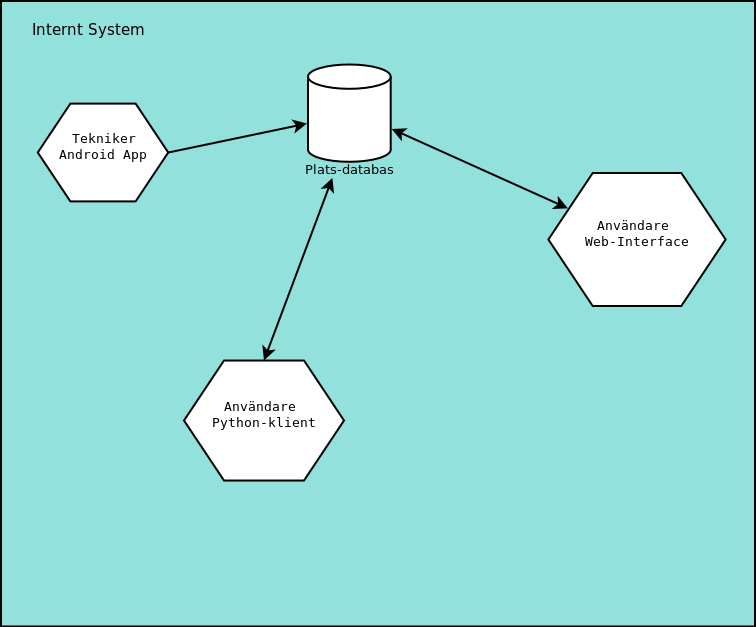
\includegraphics[width=15cm]{media/systemStruktur.png}
	\caption{Systemstruktur}
	\label{fig:systemStruktur}
\end{figure}


%\subsection{Alternativa lösningar}
% Alternativa lösningar
% Beskriv strukturen både internt (hur ert eget system är uppbyggt) och externt (vilka andra system ert system kommunicerar med). \textbf{Använd figurer} (och text)!
% \begin{itemize}
% \item Vilka delar består systemet av? (T.ex. databas, webbinterface, AI-modul, grafik...) Vilka kommunicerar med vilka, beror av vilka, innehåller vilka andra?
% \item Vilka delar fanns färdiga att använda/anpassa, vilka utvecklade ni själva? Visa tydligt, gärna grafiskt.
% \item Finns olika alternativa byggblock eller designval? Vilka är argumenten för/emot valen?
% \item Hur kommunicerar delarna, vilka protokoll och/eller dataformat används? (Beskriv mer detaljerat i senare, i Huvuddelen.)
% \item Finns det olika typer av användare/motsv? (T.ex. administratörer resp slut\-an\-vän\-dare?)
% \end{itemize}
%
% \iffalse
% \subsection{Tänk på följande}
%
% Var inte för tekniskt detaljerade här.  Tanken är att ge en översikt över systemet.  Ni behöver inte beskriva objektmetoder etc. i detalj (om de inte är nya och avgörande för resultatet). Tekniska detaljer och implementation beskriver ni snarare i Huvudddelen.
%
%
% Se till att ni använder \emph{samma terminologi} i figurer som visar systemet som i texten.
%
% Anknyt figurerna till texten på ett tydligt sätt. Om ni t.ex. har separata underrubriker som beskriver olika delar/aspekter av systemstrukturen med tillhörande figur, välj antingen en underrubrik per del i figuren eller använd helt andra underrubriker.  Annars kommer läsaren att undra var underrubriken som beskriver del X är, när det finns underrubriker för alla andra delar.
% \fi

\section{Krav och utvärderingsmetoder}\label{sec:krav}

% Vilka krav ställer ni/andra på ert resultat?
%
% hur snabbt? hur många användare? hur strömsnålt? eller vad som är relevant
% Hur ska ni utvärdera ert arbete/system (så att ni vet om/hur bra ni lyckats)?
%
% För de olika funktionaliteterna (och/eller motsv) i ert system, hur ska ni avgöra om de är tillräckligt bra utförda/implementerade? Var går gränsen för ``tillräckligt bra''? (Eller när är de ``för dåliga''?)
%
% Skilj på krav och funktionalitet. Själva funktionaliteterna har ni redan beskrivit i systemstrukturen eller huvuddelen nedan. (Har ni krav på saker ni beskriver först i huvuddelen kan ni lägga det här avsnittet efter huvuddelen.)
%
% Skriv tydliga krav \emph{som går att utvärdera}.  (Hur snabbt? Hur många användare? Hur strömsnålt? eller vad som är relevant).
%
% Beskriv hur utvärderingen ska gå till (automatiserade belastningstester, mätningar, en\-käter, fokusgrupper\ldots).
% Beskriv hur externa intressenter involveras i utvärderingen.
Kraven för det här projektet är något som vi tillsammans med kommunen har kommit fram till. Systemet där mappningen sker ska vara ett lättförståeligt och självgående system som ska förenkla förarbetet inför en flytt från kontorsbaserad verksamhet till aktivitets. Det kommer vi kunna utvärdera genom att låta en utomstående få göra sammankopplingen och sedan återkoppla om dennes upplevelse av applikationen.

Kraven på presentationen av medarbetares position är att det ska visas vilket kontor, vilken våning samt en radie på 10 meter. Detta kommer utvärderas genom ett utförligt test, med olika försvårande förhållanden.



\section{DEL x}\label{sec:delX}
\iffalse Mellan introduktion och avslutning finns ett eller sannolikt \emph{flera} avsnitt (``huvuddelen'') som innehåller själva bidraget.  Ni får själva välja passande rubriker (INTE ``Huvuddel'' eller ``Bidrag'').  Rubrikerna i huvuddelen ska tillsammans med titeln ge en idé om vad som berättas, en ``berättelse''. (Exempel: ``Algoritm för automatisk igenkänning av stora fötter'', ``Design av databasen för användardata'', ``Optimering av minnesanvändning'', ``Implementation av djupinlärningssystemet'' etc.)

Här kan ni beskriva implementationen, hur systemet används, etc.

Beskriv gärna felhantering och riskanalys: vad kan gå fel när systemet kör/används, vad kan bli följden, och hur hanteras detta?
\fi
\section{DEL x+1}
%Se avsnitt~\ref{sec:delX}.
\section{DEL x+2}
%Se avsnitt~\ref{sec:delX}.

%\ldots

\section{Utvärderingsresultat}
\iffalse Beskriv resultaten av utvärderingen, när ni tillämpar de utvärderingsmetoder ni beskrivit i avsnitt~\ref{sec:krav}, och relatera utvärderingsresultaten till kraven i samma avsnitt.
\fi

\section{Resultat och diskussion}
\iffalse Här beskriver ni först era resultat, vad ni åstadkommit.  Hur bra blev det?
Sedan granskar ni era resultat kritiskt.  Varför blev det som det blev?  Var resultaten rimliga/bra/dåliga/o\-vän\-ta\-de\ldots?
Vad hade man kunnat göra annorlunda?  Hur relaterar era resultat till liknande arbeten?

\begin{itemize}
\item Visa att utvärderingen är rimlig.
\item Visa att utvärderingen, resultatet och analysen är vetenskapliga och ingenjörsmässiga.
\end{itemize}

Relatera till mål och syften etc i avsnitt~\ref{sec:syfte}.
\fi


\section{Slutsatser}
\iffalse Här sammanfattar ni och upprepar ert bidrag (resultaten av ert projekt) och förklarar dess vikt och användning.  Vad var viktigt/nytt/intressant?  (INTE i termer av vad ni lärde er, utan för den som läser rapporten, funderar på att göra ett liknande system, vidareutveckla ert, etc.)
\fi
\section{Framtida arbete}
\iffalse Här beskriver ni potentiella framtida utvecklingar av systemet. Var finns förbättrings\-poten\-tial och vad kan man bygga vidare på? Vilka intressanta utvidgningar hann ni inte med?

Observera att risk\-be\-döm\-ning, tids\-planering, relation till kursmål \emph{inte} hör hemma i slutrapporten.
\fi
\newpage
% Here comes the bibliography/references.
\bibliography{refs}
% Use one of these:
%   IEEEtranS gives numbered references like [42] sorted by author,
%   IEEEtranSA gives ``alpha''-style references like [Lam81] (also sorted by author)
%\bibliographystyle{IEEEtranSA}

\bibliographystyle{IEEEtranS}

\newpage
\appendix %%%% markerar att resten är appendixar
\iffalse \section{Hur man gör appendix}
Appendixar kan vara bra för bilagor som enkätundersökningar, större kodavsnitt, etc.

Appendix läggs efter referenslistan, och ska börja på en ny sida. Använd \verb|\newpage| för att göra ett sidbrott där resten av nuvarande sida är tom. Skriv sen \verb|\appendix| för att markera att resten är appendix, och
 använd sen vanliga \verb|\section{}| för varje appendix, som kommer att ``numreras'' A, B, C osv.

\section{Några tips för La\TeX-användning}

Ett enkelt sätt att använda/\textbf{installera} LaTeX för MacOS är TexShop (\url{http://pages.uoregon.edu/koch/texshop}).

\textbf{Läs också i Wikibooks} (\url{http://en.wikibooks.org/wiki/LaTeX}), \textbf{missa inte} Appendix om ``Sample LaTeX documents'' (men använd alltid rapportmallen som bas).

\textbf{Citat-tecken} skriver man med \verb|``foo''| (dvs två bakåtfnuttar före, och två vanliga fnuttar efter). LaTeX gör så att det blir snyggt: ``foo''.

När man skriver på svenska behöver man ibland ``visa'' var ord (speciellt såna med med åäö) kan \textbf{avstavas} genom att använda \verb|\-| (liknande \textit{soft hyphen}): ämnesöversiktsintroduktion avstavas med några sådana instuckna på rätt ställen istället som ämnes\-över\-sikts\-intro\-duk\-tion

\begin{verbatim}
ämnes\-över\-sikts\-intro\-duk\-tion
\end{verbatim}

För att formattera \textbf{URLer} bättre (så att t.ex. radbrytning blir snyggare), skriv t.ex. \verb|\url{http://www.it.uu.se/research/group/concurrency}| i texten eller referensen.

För att \textbf{referera} till avsnitt, figurer, tabeller etc, använd \verb|\label{markör}| för att ``sätta ett märke'' i text eller figur, och \verb|\ref{markör}| för att referera till den, t.ex.
\begin{verbatim}
\section{Motivation}
\label{sec:motivation}
\end{verbatim}

följt av
\begin{verbatim}
Som vi nämnt i avsnitt~\ref{sec.motivation}...
\end{verbatim}

För att få referenser att inte hamna först efter ett \textbf{radbrott}, använd ``klister'' (icke-brytande space) \verb|såhär~\cite{fin-bok}|, där tilde-tecknet \verb|~| alltså gör ett obrytbart space. Detta är i princip också alltid rätt att använda före siffror, och förstås också före \verb|\ref{fig}|.

Använd \emph{aldrig} dubbel-backslash \verb|\\| för att få avbrott mellan stycken. Använd alltid dubbel ny rad för detta.

För att göra ett \textbf{sidbrott} där resten av sidan blir tom, använd \verb|\newpage|, inte \verb|\pagebreak|. Det senare är till för att finjustera var latex gör ett automatiskt sidbrott, inte för att avsluta en halvfull sida.

\subsection{Bib\TeX-tips}

För att hantera bibliografi (\textbf{referenser}) på ett smidigt sätt, använd BibTeX! (se \url{http://en.wikibooks.org/wiki/LaTeX/Bibliography_Management#BibTeX} och nedan om referenser.)

För att se till att BibTeX inte gör namn, förkortningar etc till lowercase, använd \verb|{}| och skriv typ
\begin{verbatim}
title = {The {DSP} of {N}ewton applied to {iOS}}
\end{verbatim}

Skriv alltid månader för publikation med de inbyggda förkortningarna, typ:
\begin{verbatim}
month = jun
\end{verbatim}
istället för \verb|{jun}| eller \verb|"jun"| eller \verb|"June"| eller \verb|"Juni"|. Då kan nämligen bibliographystyle styra hur det förkortas etc.

Ett verktyg för att hantera BibTeX-filer i MacOS är BibDesk (\url{http://bibdesk.sourceforge.net/}).


\section{Referenser}
\label{sec:referenser}

Se också kap 8.5 i Dawson~\cite{dawson:projects-in-computing}.

Det finns åtminstone tre syften med utformningen av referenserna och referenslistan.
\begin{enumerate}
\item Man ska hitta referensen (från texten) i referenslistan.
\item Man ska förstå vad som refereras (vilken typ av referens det är) så att man kan värdera den.
\item Man ska kunna hitta referensen i verkligheten.
\end{enumerate}

Använd numeriska referenser (IEEE-stil~[42]) eller nyckelordsbaserad~[Lam86], inte fotnotstil. Referenserna sorteras alfabetiskt efter författare/motsv i referenslistan. I LaTeX, använd \verb|\bibliographystyle{IEEEtranS}| eller \verb|{IEEEtranSA}| (eller liknande), se rapportmallen.

Referenserna skrivs i direkt anknytning till det som föranleder referensen (t.ex. ett påstående eller resultat), före eventuellt skiljetecken, och med ett fast mellanslag till föregående ord. I LaTeX, \verb|skriv~\cite{lam86}| för att få en ``non-breaking space''. Se också rapportmallen, och sista stycket på sid 211 i Dawson~\cite{dawson:projects-in-computing}.

Det är alltså \emph{inte} en bra approach att skriva referenserna efter ett längre stycke (som vissa verkar lära sig att göra, någonstans). Det gör det oftast otydligt vad som egentligen är hämtat från, eller styrks, av referenserna. I vissa fall kan man vilka göra en kort sammanfattning av vad en författare skriver i en artikel el.dyl., men att bara lägga på en referens sist i stycket är inte tillräckligt tydligt. Det är mycket bättre och tydligare att skriva något i stil med ``Lisa Lagom beskriver\verb|~\cite{lagom-bok}| hur X beror av Y och i sin analys visar hon i detalj hur sambandet ser ut\ldots''.

När man refererar till ``tjocka'' saker som böcker är det lämpligt att ange sidnr
(som \verb|\cite[sid 211-214]{dawson}|), men för ``tunnare'' saker behöver man bara göra det för att speciellt peka ut om man t.ex. menar en viss del av referensen (kanske den tar upp tre olika sätt att göra X och man vill peka på det 3:e, inte de första två).

För mer info om vilken info som behövs för olika typer av referenser, se avsnitt 8.5.3 i Dawson~\cite{dawson:projects-in-computing,dawson:projects-in-computing-old}. (För att referera till flera saker samtidigt (som nyss) skriver man flera BibTeX-nycklar i samma \verb|\cite|.)

Använd inte direktcitat, såvida inte den exakta formuleringen är viktig.  Skriv hellre ett referat av vad någon sagt. (Se Dawson.)

Om referenslistan huvudsakligen innehåller referenser till ``mer info'' av typen
\url{www.wordpress.org}, \url{www.w3c.org}, \url{developer.android.com}\ldots men få referenser som stöder resonemang, motivation, argument etc (jfr Workshoparna), är det antagligen ett tecken på att det finns få resonemang, motiveringar och argument som behöver stödjas. Då behöver man med största sannolikhet resonera, motivera och argumentera mera!

Även om en referens har en URL till själva texten är det inte nödvändigtvis en webbreferens, utan ibland en artikel/bok el.dyl som råkar vara tllgänglig på nätet. Den ska då beskrivas som artikel/bok/el.dyl, men förstås gärna med URLen.

\section{Formler, figurer, bilder, kod}
\label{sec:forml-figur-bild}

Formler och/eller ekvationer måste beskrivas.  Det betyder t.ex. att varje symbol måste vara förklarad i texten.

I engelsk text skriver man ``Figure 3'', inte ``figure 3'', eftersom det fungerar som ett namn på figuren (och motsvarande för Table osv).

Alla figurer och bilder som inte är era egna måste ha referenser.

Om ni inkluderar kodsnuttar, se till att de är relevanta och kommenterade, så att man förstår.  Alternativt, för korta snuttar: ge motsvarande förklaring i texten.
Använd vettigt latex-bibliotek för kod, t.ex. \texttt{listings}.

\section{Språk och grammatik}
\label{sec:sprak-och-grammatik}

\begin{itemize}
\item    Det är OK att skriva ``Vi''!

\item    \textbf{Inte alla läsare är män}.  Skriv därför inte ``han'', ``hans'', ``denne'' etc.  Använd könsneutrala pronomen eller ord som ``vederbörande'', ``användaren'' etc.

\item    \textbf{Undvik talspråk} ``så'', ``två stycken saker'', ``ifrån'', ``utav'', ``vart'', ``kommer göra/vara'' (istället för ``kommer att göra/vara'', \ldots \textbf{Kolla på Wikipedia-sidan} ``Vanliga språkfel'' (länk i vänsterkanten i SP).

\item    Undvik värderande uttryck som enkelt, uppenbart.

\item    Semikolon är \textbf{inte} en variant av kolon eller komma; semikolon kan endast användas där ni normalt sett skulle använt punkt, men vill fortsätta på samma mening. För att undvika problem, undvik semikolon helt.

\item    Skriv inte meningar som börjar med ``Detta på grund av'' eller ``Detta eftersom\ldots' -- det blir ofta inte fullständiga meningar och det är ofta inte klart vad ``detta'' syftar på.

\item    Använd inte framtid; skriv rapporten i nu- eller dåtid och var konsekventa (Vi gör\ldots eller Vi har gjort\ldots, inte Vi kommer att göra\ldots)

\item    \textbf{Förklara begrepp innan ni använder dem}, hänvisa inte \emph{bara} läsaren till ett senare avsnitt (men ni kan naturligtvis också hänvisa till mer detaljerade förklaringar som kommer senare i texten).  Första gången ett begrepp nämns måste alltså åtminstone en kort förklaring finnas.

\item    När ni introducerar nya koncept (sådant ni inte har diskuterat tidigare), gör inte det ``i förbifarten'', utan se till att ni \textbf{förklarar ordentligt}.  Alltså: ``Vi använder X (ett häftigt nytt programmeringsspråk) för att göra Y'' fungerar inte.  Beskriv först konceptet ni använder, och använd det sedan.  Typ ``X är ett viktigt nytt programmeringsspråk.  Vi använder X för att göra Y.''

\item    \textbf{Var konsekventa} med hur ni skriver förkortningar och begrepp (c++ eller C++, android och Android t.ex.) Tumregel: namn skrivs med inledande stor bokstav (Android, inte android), förkortningar med stora bokstäver (XML, inte Xml).
\item    Använd inte olika synonymer för det ni har utvecklat (tjänsten/projektet/systemet), utan bestäm er för vad det är ni har gjort.

\item    Det kan vara bra att kursivera nya begrepp första gången de används, men normalt bör man inte kursivera \emph{alla} förekomster.

\item    Efter uttryck som ``för det första\ldots'', ``one alternative is\ldots'' måste följa ``för det andra\ldots'' ``another alternative'' (inte ``slutligen'', ``dels'', ``another \underline{option}'' eller något annat).  Tänk också på ``firstly \ldots secondly'' resp. ``first \ldots second'', inte ``first \ldots secondly'' eller något annat.

\item    Var försiktig med uttryck som ``this approach'', ``detta system'', etc. och kontrollera att det är uppenbart vad detta/this refererar till. Be någon icke-gruppmedlem läsa och kolla!

\item    De av er som skriver på engelska: ni MÅSTE använda korrekta verbformer beroende på om subjektet är en eller flera saker (``it has'' men ``they have'').
\end{itemize}
\fi
\section{Tidsplan}
\subsection{Gantt-diagram}

\begin{figure}[h]
	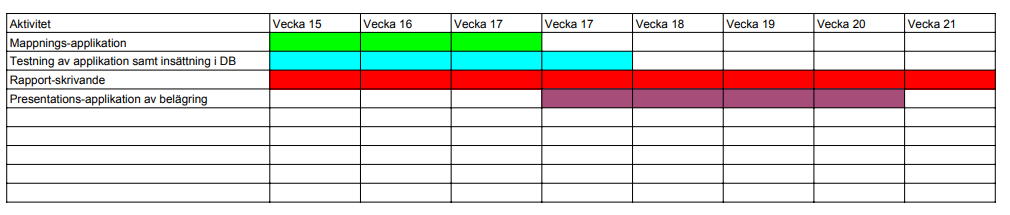
\includegraphics[width=15cm]{media/GANTT.png}
	\caption{GANTT Diagram}
	\label{}
\end{figure}

\subsection{Arbetsbelastning}
Vi har planerat att arbeta omkring 8 timmar per dag varav hälften tillsammans och hälften var för sig. Anledningen till detta är då mycket av det administrativa kan göras på egen hand samt vissa delar av programmernadet. Dock är det bra att arbeta tillsammans också då kommunikationen blir enklare samt förekommer avstämningsmöten varenda dag.

\subsection{Feedback från videopitch}
Den feedback vi fick från videopitcharna gick till det mesta ut på att vara tydligare rörande vad aktivitetsbaserade arbetsplatser egentligen innebär.
Vi har försökt klargöra innebörden av en aktivitetsbaserad arbetsplats i framförallt abstract och avsnittet bakgrund i rapporten. Förhoppningsvis är förklaringen nu tillräckligt utförlig för att läsaren enkelt ska förstå vad vårt projekt syftar till.


\subsection{Milstolpar}
Vi har delat upp våra milstolpar i två delar. En för systemt och en för rapporten. Till rapporten valde vi att använda milstolparna som vi fick av kursansvariga, dvs de inlämningar som ska in ska in i tid. Till systemet har vi följande milstolpar:
\begin{itemize}
	\item 22/3 Projektbeskrivning klar.
	\item 27/3 Läst grundläggande om relativ information angående projektet. Bland annat positionering, Wifi skanning, Kotlin programmering, android utveckling.
	\item 3/4 Få första android applikationen att kunna skanna av ett nätverk och få relativ information och kunna spara informationen på ett lämpligt sätt (i en .csv fil).
	\item 17/4 Få tillgång till Kommunen lokaler för att testa första android applikationen och få tillgång till Skype for Buisness (SFB) databasen för att kunna fortsätta arbeta med skriptet för att populera dess databas.
 	\item 25/4 Ha ett fungerande skript som kan populera  SFB databasen.
	\item 7/5 Första prototyp för android applikationen som ska visualisera arbetsplatsen med relativ data. Samt få den godkänd av Uppsala kommun.
	\item 14/5 Ha alla delsystem färdiga.
	\item 21/5 Koppla samman alla delsystem.
	\item 28/5 Ett fungerande system. Programmerings stop.
\end{itemize}

%TODO : 1) Hur ska vi kunna separera AP via våningar? (Vart ska det stå?)
%TODO : 2) Fingerprinting varför bara en del? (Kommer inte ihåg vad jag menade med ni kanske gör)
%TODO : 3) Kommunen hur ser det ut?
%TODO : 4) Skype 4 Buisness, Skriva att vi skiter i det och varför vi skiter i det? (Vart ska det stå?)
\end{document}
